\documentclass[11pt,a4paper]{article}

% --- Pakete ---
\usepackage[utf8]{inputenc}
\usepackage[T1]{fontenc}
\usepackage[ngerman]{babel}
\usepackage{lmodern}
\usepackage[a4paper, top=2.2cm, bottom=2.2cm, left=2.4cm, right=2.4cm]{geometry}
\usepackage{amsmath, amssymb}
\usepackage{siunitx}
\sisetup{
  output-decimal-marker={,},
  separate-uncertainty=true,
  per-mode=symbol,
  range-units=single,
  range-phrase=\,--\,,
  exponent-product=\cdot
}
\usepackage{graphicx}
\usepackage{subcaption}
\usepackage{booktabs}
\usepackage{caption}
\captionsetup{font=small, labelfont=bf}
\usepackage{float}
\usepackage{microtype}
\usepackage{hyperref}
\hypersetup{hidelinks}
\usepackage{enumitem}
\setlist{nosep, leftmargin=*}
\setlength{\parskip}{4pt}
\setlength{\parindent}{0pt}

% --- Titel ---
\title{\vspace{-1cm}\textbf{Trägheitsmoment (TRM)}\\[2pt]
\large Physikalisches Praktikum --- TU München}
\author{Tamino Bruckmoser, Sebastian Richter \\ Team \emph{Tamastian}}
\date{Durchführung: 5. Mai 2026}

\begin{document}

\maketitle

\noindent
\begin{tabular}{ll}
  Kursnummer:    & 5 \\
  Teamnummer:    & 5-07 \\
  Versuchsname:  & Trägheitsmoment (TRM) \\
  Durchführung:  & 5.\,Mai 2026 \\
  Ausarbeitung:  & 5.\,Mai 2026 (v1.0) \\
\end{tabular}

\vspace{1ex}\hrule\vspace{0.5ex}
\tableofcontents
\vspace{0.5ex}\hrule

% =========================================================
\section{Einleitung}
% =========================================================
Ziel des Versuchs ist die Bestimmung des Trägheitsmoments einer
Puppe und eines Menschen aus Drehschwingungen sowie der Vergleich
mit drei verschiedenen Modellrechnungen. Hierfür werden zwei
Drehapparaturen mit jeweils statischer und dynamischer Methode
charakterisiert.

% =========================================================
\section{Grundlagen}
% =========================================================
Das Trägheitsmoment $J$ eines Massepunkts in Bezug auf eine
Rotationsachse ist gemäß \cite{anleitung}
\begin{equation}
  J = m\,r^{2}, \tag{1}
\end{equation}
wobei $r$ der Abstand zur Rotationsachse ist. Für ausgedehnte Körper
folgt durch Integration $J = \int r^{2}\,\rho\,\mathrm{d}V$. Liegt
die Drehachse nicht durch den Schwerpunkt, gilt der Steiner-Satz
\begin{equation}
  J_{A} = J_{S} + m\,r_{a}^{2}. \tag{2}
\end{equation}

Eine harmonische Drehschwingung um eine Spiralfeder mit
Winkelrichtgröße $D^{*}$ besitzt die Schwingungsdauer
\begin{equation}
  T = 2\pi\,\sqrt{\frac{J}{D^{*}}}. \tag{3}
\end{equation}
Setzt man die Apparatur mit Eigenträgheitsmoment $J_{0}$ um eine
zusätzliche Last $J_{z}$, folgt
\begin{equation}
  T^{2} = \frac{4\pi^{2}}{D^{*}}\,(J_{0} + J_{z}). \tag{4}
\end{equation}
Im statischen Verfahren wird das rückstellende Drehmoment
$M = -D^{*}\varphi$ direkt gemessen; die Steigung der Geraden in
der Auftragung $M(\varphi)$ liefert $-D^{*}$. Die ausführliche
Herleitung findet sich in \cite{anleitung}; eine Zusammenstellung
der Trägheitsmomente einfacher Körper sowie der Massenanteile der
Körperteile ist ebenfalls dort gegeben.

Für die Extrapolation Puppe~$\to$~Mensch gilt unter Annahme
geometrisch ähnlicher Körper
\begin{equation}
  J_{\mathrm{Mensch}} = \frac{M}{m}\Big(\frac{L}{l}\Big)^{2} J_{\mathrm{Puppe}}, \tag{5}
\end{equation}
und unter zusätzlicher Annahme gleicher Dichte
\begin{equation}
  J_{\mathrm{Mensch}} = \Big(\frac{L}{l}\Big)^{5} J_{\mathrm{Puppe}}. \tag{6}
\end{equation}

\paragraph{Vorüberlegungen.}
Aus $M = F\,r\,\cos\theta$ folgt für eine Winkelabweichung
$\theta$ aus der Tangentialrichtung ein relativer Drehmomentfehler
$1-\cos\theta$. Die Forderung $<\SI{1}{\percent}$ ergibt
$\theta \le \SI{8{,}1}{\degree}$. Behandelt man Mensch bzw.\ Puppe als
homogenen Zylinder mit Radius $R$, so liefert der Steiner-Satz aus
$d^{2} \le 0{,}1\,R^{2}/2$ den maximal zulässigen Achsenversatz
$d_{\max} = R/\sqrt{20}$. Mit dem Hüftumfang
$U = \SI{83}{\centi\metre}$ folgt für den Menschen
$d_{\max} \approx \SI{3{,}0}{\centi\metre}$, für die Puppe
($D=\SI{5{,}5}{\centi\metre}$) $d_{\max}\approx\SI{6}{\milli\metre}$.

% =========================================================
\section{Experimentelles Vorgehen}
% =========================================================
Verwendet wurden zwei Drehapparaturen: eine kleine Drehachse mit
Spiralfeder und Hilfsstab (Hebelarm der Federwaage
$r=\SI{15{,}5}{\centi\metre}$) für die Puppen-Messung, sowie der
große Drehteller (Drehteller~Nr.\,3, Aluminium, Durchmesser
$\SI{60}{\centi\metre}$, Dicke $\SI{2}{\centi\metre}$) für die
Mensch-Messung; Hebelarm bei der statischen Bestimmung
$r=\SI{30}{\centi\metre}$ (Tellerrand).

\paragraph{Statische Bestimmung der Winkelrichtgröße.}
Bei festgehaltenem Drehkörper wurde mit einer Federwaage die
zur Halterung tangentiale Rückstellkraft $F$ bei vorgegebenen
Auslenkungswinkeln gemessen --- bei der kleinen Drehachse in
$\SI{45}{\degree}$-Schritten von $\pm\SI{180}{\degree}$, beim
großen Drehteller in $\SI{10}{\degree}$-Schritten von
$\pm\SI{90}{\degree}$, jeweils in beiden Drehrichtungen. Die
Rohdaten enthalten Beträge der Federkraft; das Vorzeichen
des rückstellenden Drehmoments wird über $\mathrm{sgn}(-\varphi)$
rekonstruiert.

\paragraph{Dynamische Bestimmung von $D^{*}$ und $J_{0}$ (kleine Drehachse).}
Bei eingestecktem Hilfsstab ohne Zusatzgewichte sowie mit einem
Gewichtepaar (Gesamtmasse $\SI{97{,}4}{\gram}$, Höhe
$\SI{0{,}5}{\centi\metre}$, Durchmesser $\SI{2{,}7}{\centi\metre}$) in
fünf verschiedenen Abständen $r=0,5,10,15,\SI{20}{\centi\metre}$
wurde jeweils die Halbschwingungsdauer für Auslenkungen
$\varphi_{0}\approx\SI{90}{\degree}$ und $\SI{135}{\degree}$
\emph{mit einer elektronischen Lichtschranke}
(digitale Anzeige, Auflösung $\SI{1}{\milli\second}$) erfasst. Die
volle Periode $T$ folgt durch Verdopplung.

\paragraph{Messung der Puppe.}
Halbschwingungsdauer der mit dem Hilfsstab verbundenen Puppe
($m = \SI{183}{\gram}$, $l=\SI{32}{\centi\metre}$, Hüftdurchmesser
$\SI{5{,}5}{\centi\metre}$ angelegt bzw. $\SI{3}{\centi\metre}$ mit
Spannweite $\SI{32}{\centi\metre}$ ausgestreckt) bei
$\varphi_{0}\approx\SI{90}{\degree}$ und $\SI{135}{\degree}$ in
beiden Haltungen --- ebenfalls mit der Lichtschranke der kleinen
Drehachse.

\paragraph{Großer Drehteller / Mensch.}
Die Schwingungsdauer am großen Drehteller wurde gemäß
Versuchsanleitung mit \emph{Hand\-stopp\-uhr} (Computer-Anzeige,
Auflösung $\SI{10}{\milli\second}$) erfasst.
Ohne Person wurde über 23~Halbschwingungen ($t = \SI{38{,}97}{\second}$)
die mittlere Halbschwingungsdauer bestimmt; die volle Periode
folgt durch Verdopplung. Mit der Versuchsperson
($M=\SI{70}{\kilogram}$, $H=\SI{183}{\centi\metre}$) wurden
für jede der beiden Haltungen drei unabhängige Messungen über
jeweils 4 oder 5 \emph{ganze} Schwingungen durchgeführt. Zusätzlich wurden die Körpermaße (Kopfumfang
$\SI{59}{\centi\metre}$, Hüftumfang $\SI{83}{\centi\metre}$, sowie
Längen und Umfänge der Glieder) zur Modellrechnung aufgenommen
(Notation Länge\,$\times$\,Umfang in cm: Oberarm 32$\times$30,
Unterarm 47$\times$18, Oberschenkel 38$\times$43, Unterschenkel
47$\times$32).

% =========================================================
\section{Ergebnisse}
% =========================================================

\subsection{Kleine Drehachse (Puppe)}
\paragraph{Statische Bestimmung von $D^{*}$.}
Abbildung~\ref{fig:stat_puppe} zeigt das aus
$M = F\cdot r\cdot\mathrm{sgn}(-\varphi)$ bestimmte rückstellende
Drehmoment in Abhängigkeit von $\varphi$. Eine ungewichtete
lineare Regression liefert die Steigung $a_{1}=-D^{*}_{\mathrm{stat}}$.
Unter Berücksichtigung der Skalierungsunsicherheit der Federwaage
(\SI{1}{\percent}) und der Hebelarm-Unsicherheit
($u(r)=\SI{1}{\milli\metre}$) ergibt sich
\begin{equation}
  D^{*}_{\mathrm{stat}} = \SI{24{,}5(7)}{\milli\newton\metre\per\radian}. \tag{7}
\end{equation}
Der Achsenabschnitt liegt mit $\SI{-3{,}8(12)}{\milli\newton\metre}$ ca.\
$3\sigma$ neben dem Ursprung, was auf einen kleinen systematischen
Offset (z.\,B.\ Hysterese der Spiralfeder) hindeutet, die
Steigung wird dadurch jedoch nicht beeinflusst.

\begin{figure}[H]
  \centering
  \begin{subfigure}[t]{0.49\textwidth}
    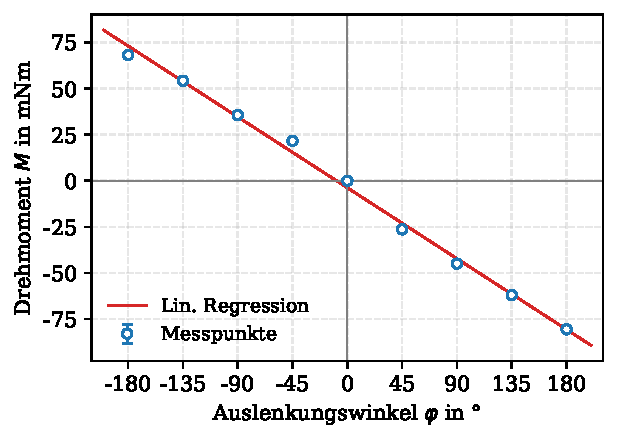
\includegraphics[width=\linewidth]{abb_statisch_puppe.pdf}
    \caption{Statische Bestimmung: $M(\varphi)$ an der kleinen Drehachse.}
    \label{fig:stat_puppe}
  \end{subfigure}\hfill
  \begin{subfigure}[t]{0.49\textwidth}
    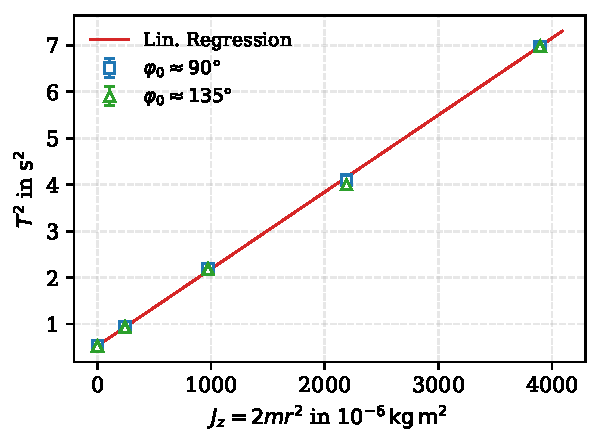
\includegraphics[width=\linewidth]{abb_dynamisch_puppe.pdf}
    \caption{Dynamische Bestimmung: $T^{2}$ vs.\ $J_{z}=2mr^{2}$.}
    \label{fig:dyn_puppe}
  \end{subfigure}
  \caption{Auswertung der kleinen Drehachse. Beide Methoden liefern
    konsistente Werte für $D^{*}$.}
\end{figure}

\paragraph{Dynamische Bestimmung von $D^{*}$ und $J_{0}$.}
Die Ausdehnung der Gewichte ist gegenüber $r^{2}$ vernachlässigbar:
mit $R=\SI{1{,}35}{\centi\metre}$ und $h=\SI{0{,}5}{\centi\metre}$
beträgt der Eigenanteil eines Gewichts
$m\bigl(R^{2}/4 + h^{2}/12\bigr) \approx \SI{4{,}6e-6}{\kilogram\metre\squared}$, also
$\le\SI{0{,}5}{\percent}$ schon bei $r=\SI{5}{\centi\metre}$. Aus
Gleichung~(4) folgt mit $J_{z}=2mr^{2}$ ein linearer Zusammenhang
$T^{2}(J_{z})$. Die gewichtete Regression über beide
Auslenkungssätze (Abbildung~\ref{fig:dyn_puppe}) ergibt Steigung
$a_{1}=\SI{1657(5)}{\second\squared\per(\kilogram\metre\squared)}$ und
Achsenabschnitt $a_{0}=\SI{0{,}530(5)}{\second\squared}$, woraus
\begin{align}
  D^{*}_{\mathrm{dyn}} &= \frac{4\pi^{2}}{a_{1}} = \SI{23{,}83(7)}{\milli\newton\metre\per\radian}, \tag{8}\\
  J_{0}                &= \frac{a_{0}}{a_{1}} = \SI{320(3)e-6}{\kilogram\metre\squared}. \tag{9}
\end{align}
$D^{*}_{\mathrm{stat}}$ und $D^{*}_{\mathrm{dyn}}$ stimmen mit einer
Differenz von $\SI{0{,}64}{\milli\newton\metre\per\radian}$
($\approx 0{,}9\sigma$) innerhalb $1\sigma$ überein. Da
$D^{*}_{\mathrm{dyn}}$ aufgrund der elektronischen Zeitmessung mit
einer um etwa eine Größenordnung kleineren Unsicherheit behaftet ist
und unmittelbar in der gleichen Schwingungsmessung steckt, wird im
Folgenden mit diesem Wert gerechnet.

\paragraph{Trägheitsmoment der Puppe.}
Mit $J_{\mathrm{Puppe}} = (D^{*}/4\pi^{2})\,(T^{2}-T_{0}^{2})$ ergibt
sich aus den Schwingungsdauern (Tabelle~\ref{tab:puppe})
\begin{align}
  J_{\mathrm{Puppe}}^{\text{angelegt}}    &= \SI{77{,}0(11)e-6}{\kilogram\metre\squared}, \tag{10}\\
  J_{\mathrm{Puppe}}^{\text{ausgestreckt}} &= \SI{280{,}0(64)e-6}{\kilogram\metre\squared}. \tag{11}
\end{align}
Das Verhältnis ergibt
$J_{\text{ausgestreckt}}/J_{\text{angelegt}} = 3{,}63 \pm 0{,}10$.
Der Lichtschranken-Trigger liefert einen Typ-B-Beitrag von
$\SI{0{,}4}{\milli\second}$ pro Periode, sodass die
Gesamtunsicherheit der Puppen-Trägheitsmomente von der
Federwaagen-Skalierung (über $D^{*}_{\mathrm{dyn}}$) und --- in der
ausgestreckten Haltung --- von der Streuung der beiden
Auslenkungsmessungen
(Standardabweichung $\sim\SI{4}{\milli\second}$ auf $T$) dominiert
wird.

\subsection{Großer Drehteller (Mensch)}
\paragraph{Statische Bestimmung.}
Abbildung~\ref{fig:stat_drehteller} zeigt $M(\varphi)$ am
Drehteller. Lineare Regression liefert
\begin{equation}
  D^{*}_{\mathrm{stat}} = \SI{2{,}30(5)}{\newton\metre\per\radian}. \tag{12}
\end{equation}
Die Asymmetrie der Beträge $\lvert F(\varphi=\SI{+90}{\degree})\rvert =
\SI{10}{\newton}$ vs.\ $\lvert F(\SI{-90}{\degree})\rvert = \SI{13{,}5}{\newton}$
ist als Reibungs-Hysterese deutlich erkennbar (vgl. Achsenabschnitt
$a_{0}\approx \SI{0{,}31}{\newton\metre}$, entsprechend
$F_{\mathrm{Reib}}\approx \SI{1}{\newton}$); die Steigung wird
durch die zweiseitige Messung kaum verfälscht.

\begin{figure}[H]
  \centering
  \begin{subfigure}[t]{0.49\textwidth}
    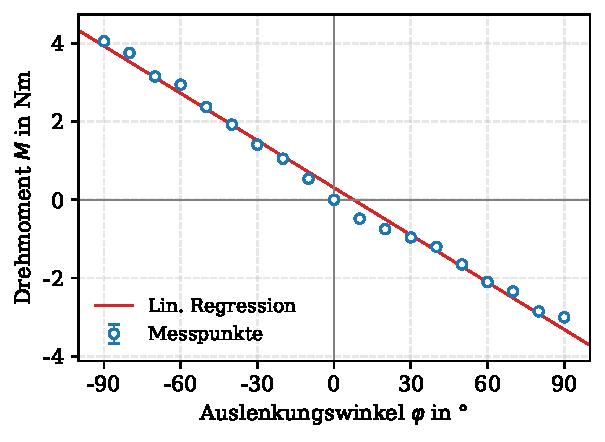
\includegraphics[width=\linewidth]{abb_statisch_drehteller.pdf}
    \caption{$M(\varphi)$, Drehteller. Asymmetrie um $\varphi=0$ deutet auf Reibung hin.}
    \label{fig:stat_drehteller}
  \end{subfigure}\hfill
  \begin{subfigure}[t]{0.49\textwidth}
    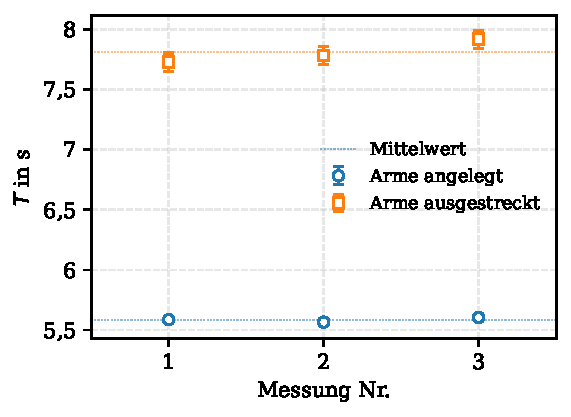
\includegraphics[width=\linewidth]{abb_schwingungsdauer_mensch.pdf}
    \caption{Drei Wiederholungen je Haltung, mit Mittelwerten.}
    \label{fig:schw_mensch}
  \end{subfigure}
  \caption{Messungen am großen Drehteller.}
\end{figure}

\paragraph{Eigenträgheitsmoment $J_{0}$ und dynamische
Charakterisierung.}
Aus der geometrischen Berechnung der Aluminium-Scheibe
($\rho=\SI{2{,}7}{\gram\per\cubic\centi\metre}$, $D=\SI{60}{\centi\metre}$,
$h=\SI{2}{\centi\metre}$, Mittelstange $\SI{75}{\centi\metre}\times\SI{2{,}5}{\centi\metre}$)
folgt
\begin{equation}
  J_{0} = \tfrac{1}{2}m R^{2} = \SI{0{,}69(4)}{\kilogram\metre\squared}, \tag{13}
\end{equation}
wobei der Beitrag der zentralen Stange ($\SI{7{,}8e-5}{\kilogram\metre\squared}$)
vernachlässigt wird. Die Halbschwingungsdauer ohne Person beträgt
$T_{0,1/2}=\SI{1{,}694(3)}{\second}$, also
$T_{0}=2\,T_{0,1/2}=\SI{3{,}389(6)}{\second}$. Daraus
\begin{equation}
  D^{*}_{\mathrm{dyn}} = \frac{4\pi^{2}\,J_{0}}{T_{0}^{2}} = \SI{2{,}36(13)}{\newton\metre\per\radian}. \tag{14}
\end{equation}
$D^{*}_{\mathrm{stat}}$ und $D^{*}_{\mathrm{dyn}}$ stimmen innerhalb
$1\sigma$ überein. Im Folgenden wird mit dem dynamischen Wert
gerechnet, da $J_{0}$ in beiden Größen auf gleiche Weise eingeht
und sich somit Anteile des Hebelarm-Fehlers herauskürzen.

\paragraph{Trägheitsmoment des Menschen.}
Aus den drei Wiederholungen je Haltung
(Abbildung~\ref{fig:schw_mensch}, Tabelle~\ref{tab:mensch}) folgen
für die volle Periode
\begin{align}
  T_{\mathrm{angelegt}}    &= \SI{5{,}585(17)}{\second}, \tag{15}\\
  T_{\mathrm{ausgestreckt}} &= \SI{7{,}81(8)}{\second}. \tag{16}
\end{align}
Mit $J_{\mathrm{Mensch}}=(D^{*}/4\pi^{2})(T^{2}-T_{0}^{2})$ folgen
\begin{align}
  J_{\mathrm{Mensch}}^{\text{angelegt}}    &= \SI{1{,}18(6)}{\kilogram\metre\squared}, \tag{17}\\
  J_{\mathrm{Mensch}}^{\text{ausgestreckt}} &= \SI{2{,}96(17)}{\kilogram\metre\squared}. \tag{18}
\end{align}
Das Verhältnis ist
$J_{\text{ausgestreckt}}/J_{\text{angelegt}} = 2{,}51 \pm 0{,}20$.

\subsection{Theoretische Trägheitsmomente des Menschen}
Modelliert man den Menschen als zentralen Zylinder (Rumpf,
Hüftumfang $\SI{83}{\centi\metre}$) mit Kopf-Kugel
($\SI{59}{\centi\metre}$ Umfang) und vier seitlichen Zylindern
für die Glieder, so liefert die Summe der Einzel-Trägheitsmomente
inkl.\ Steiner-Satz
\begin{align}
  J_{\mathrm{theo}}^{\text{angelegt}}    &= \SI{0{,}68(7)}{\kilogram\metre\squared}, \tag{19}\\
  J_{\mathrm{theo}}^{\text{ausgestreckt}} &= \SI{2{,}94(29)}{\kilogram\metre\squared}. \tag{20}
\end{align}
Bei den ausgestreckten Armen dominiert der Steiner-Beitrag der
Arme. Die einfache Zylindernäherung
$J_{\mathrm{Zyl}} = M\,U^{2}/(8\pi^{2}) = \SI{0{,}611(9)}{\kilogram\metre\squared}$
(\cite{anleitung}, Gl.~17 dort) unterschätzt das gemessene $J$
noch geringfügig stärker, weil sie die seitlichen Glieder nicht
berücksichtigt.

Die Extrapolation aus der Puppe (angelegte Haltung) liefert mit
Gleichung~(5)
$J_{\text{extra}}^{(5)} = \SI{0{,}96(3)}{\kilogram\metre\squared}$ und
mit Gleichung~(6)
$J_{\text{extra}}^{(6)} = \SI{1{,}4(3)}{\kilogram\metre\squared}$.
Der Vergleich aller Werte ist in
Tabelle~\ref{tab:vergleich_mensch} und
Abbildung~\ref{fig:vergleich_mensch} dargestellt.

\begin{table}[H]
\centering
\caption{Zusammenfassung der Trägheitsmomente des Menschen.}
\label{tab:vergleich_mensch}
\small
\begin{tabular}{lcc}
\toprule
Methode & $J_{\text{angelegt}}\,[\si{\kilogram\metre\squared}]$
        & $J_{\text{ausgestreckt}}\,[\si{\kilogram\metre\squared}]$ \\
\midrule
Messung (mit $D^{*}_{\mathrm{dyn}}$)   & $1{,}18 \pm 0{,}06$ & $2{,}96 \pm 0{,}17$ \\
Messung (mit $D^{*}_{\mathrm{stat}}$)  & $1{,}15 \pm 0{,}03$ & $2{,}89 \pm 0{,}10$ \\
Modell (Zylinder + Kugel)              & $0{,}68 \pm 0{,}07$ & $2{,}94 \pm 0{,}29$ \\
Zylinder-Näherung (vgl.\ \cite{anleitung})& $0{,}611 \pm 0{,}009$ & --- \\
Extrapolation Gl.~(5)                  & $0{,}96 \pm 0{,}03$ & --- \\
Extrapolation Gl.~(6)                  & $1{,}4 \pm 0{,}3$   & --- \\
\bottomrule
\end{tabular}
\end{table}

\begin{figure}[H]
  \centering
  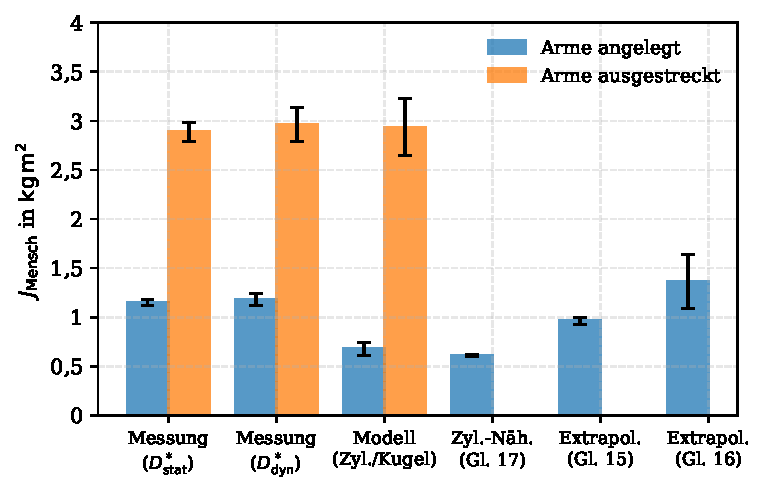
\includegraphics[width=0.78\textwidth]{abb_vergleich_mensch.pdf}
  \caption{Vergleich aller bestimmten und gemessenen Trägheitsmomente des Menschen.}
  \label{fig:vergleich_mensch}
\end{figure}

% =========================================================
\section{Diskussion}
% =========================================================
\paragraph{Konsistenz der Puppen-Apparatur.}
Die statische und dynamische Bestimmung von $D^{*}$ stimmen mit
$\SI{24{,}5(7)}{\milli\newton\metre\per\radian}$ vs.\
$\SI{23{,}83(7)}{\milli\newton\metre\per\radian}$ innerhalb $1\sigma$
überein --- die kleine Drehachse ist sauber kalibriert. Die
elektronische Zeitmessung mit Lichtschranke liefert eine
Typ-B-Unsicherheit von
$u_{\mathrm{B}}(T)=2d/(2\sqrt{3})\,/\sqrt{2}\approx\SI{0{,}4}{\milli\second}$
(digitale Anzeige $d=\SI{1}{\milli\second}$, Rechteckverteilung), die
gegenüber den übrigen Beiträgen vernachlässigbar ist. Die
Restunsicherheit der Puppen-Trägheitsmomente
($\SI{77{,}0(11)e-6}{\kilogram\metre\squared}$ angelegt,
$\SI{280{,}0(64)e-6}{\kilogram\metre\squared}$ ausgestreckt) wird
daher von $D^{*}_{\mathrm{dyn}}$ (Federwaage, ca.\ \SI{0{,}3}{\percent})
sowie bei der ausgestreckten Haltung von der Streuung der zwei
Auslenkungssätze bestimmt. Die Puppe als reiner Zylinder mit
$D=\SI{5{,}5}{\centi\metre}$ liefert theoretisch
$J = \SI{69e-6}{\kilogram\metre\squared}$; der Messwert in der
angelegten Haltung liegt $\sim\SI{8e-6}{\kilogram\metre\squared}$
darüber und macht den Beitrag von Kopf, Armen und ausragenden
Gliedern direkt sichtbar.

\paragraph{Konsistenz beim großen Drehteller.}
$D^{*}_{\mathrm{stat}}=\SI{2{,}30(5)}{\newton\metre\per\radian}$
und $D^{*}_{\mathrm{dyn}}=\SI{2{,}36(13)}{\newton\metre\per\radian}$
sind innerhalb $1\sigma$ verträglich; das geometrisch berechnete
$J_{0}$ ist also mit der gemessenen Schwingungsdauer konsistent.
Die Reibungs-Asymmetrie der statischen Messung
($F_{\mathrm{Reib}} \approx \SI{1}{\newton}$, vgl.\ Achsenabschnitt
$a_{0}\approx\SI{0{,}31}{\newton\metre}$) ist durch das
zweiseitige Verfahren weitgehend kompensiert. Im Folgenden wird
mit $D^{*}_{\mathrm{dyn}}$ gerechnet, dessen Federwaagen-Beitrag
über die geometrische $J_{0}$-Bestimmung umgangen wird.

\paragraph{Vergleich Messung vs.\ Modell.}
In der ausgestreckten Haltung stimmt die Messung
$\SI{2{,}96(17)}{\kilogram\metre\squared}$ innerhalb $1\sigma$ mit der
Modellrechnung $\SI{2{,}94(29)}{\kilogram\metre\squared}$
überein --- der Steiner-Anteil der ausgestreckten Arme dominiert
das Trägheitsmoment, und das Modell beschreibt diesen Beitrag
korrekt. In der angelegten Haltung
($\SI{1{,}18(6)}{\kilogram\metre\squared}$ Messung vs.\
$\SI{0{,}68(7)}{\kilogram\metre\squared}$ Modell) liegt der
Modellwert ca.\ $5\sigma$ unterhalb der Messung. Das Zylinder-Modell
unterschätzt $J$ in der angelegten Haltung systematisch, weil es
die Schultern-Hüft-Asymmetrie und die nicht-streng-zylindrische
Form des Rumpfes nicht erfasst; auch atmungs- und muskelbedingte
Schwerpunktsbewegungen während der Schwingung können effektiv $J$
erhöhen. Die Extrapolation aus der Puppe nach Gleichung~(6) liefert
$\SI{1{,}4(3)}{\kilogram\metre\squared}$, was mit dem Messwert
innerhalb $1\sigma$ übereinstimmt. Die Extrapolation nach
Gleichung~(5) ergibt $\SI{0{,}96(3)}{\kilogram\metre\squared}$ und
liegt damit ca.\ $3\sigma$ unterhalb der Messung. Da Gl.~(5)
geometrische Ähnlichkeit zwischen Puppe und Mensch voraussetzt, die
Puppe aber proportional einen schlankeren Rumpf und längere
Gliedmaßen besitzt, ist diese Abweichung als Modellfehler zu
verstehen: der reine $L^{2}$-Skalierungsfaktor unterschätzt das
tatsächliche $J$ des Menschen. Quantitativ belegt das auch das
Verhältnis $J_{\text{ausgestr.}}/J_{\text{angelegt}}$, das für die
Puppe $3{,}63(10)$, für den Menschen aber nur $2{,}51(20)$ beträgt
--- die Geometrie ist eben nicht ähnlich. Literaturwerte für das Trägheitsmoment des Menschen
um die Längsachse liegen je nach Körperbau zwischen $1$ und
$\SI{2}{\kilogram\metre\squared}$ (angelegt) und bei $\sim\SI{3}{}$
bis $\SI{5}{\kilogram\metre\squared}$ (ausgestreckt)
\cite{demtroeder} und stützen das Messergebnis.

% =========================================================
\section{Zusammenfassung}
% =========================================================
\begin{itemize}
  \item Kleine Drehachse (Zeitmessung mit Lichtschranke):
        $D^{*} = \SI{23{,}83(7)}{\milli\newton\metre\per\radian}$,
        $J_{0} = \SI{320(3)e-6}{\kilogram\metre\squared}$.
  \item Trägheitsmoment der Puppe:
        $J_{\text{angelegt}} = \SI{77{,}0(11)e-6}{\kilogram\metre\squared}$,
        $J_{\text{ausgestreckt}} = \SI{280{,}0(64)e-6}{\kilogram\metre\squared}$.
        Verhältnis $3{,}63 \pm 0{,}10$.
  \item Großer Drehteller: $D^{*}_{\mathrm{stat}} = \SI{2{,}30(5)}{\newton\metre\per\radian}$
        und $D^{*}_{\mathrm{dyn}} = \SI{2{,}36(13)}{\newton\metre\per\radian}$
        stimmen innerhalb $1\sigma$ überein;
        $J_{0} = \SI{0{,}69(4)}{\kilogram\metre\squared}$.
  \item Trägheitsmoment des Menschen:
        $J_{\text{angelegt}} = \SI{1{,}18(6)}{\kilogram\metre\squared}$,
        $J_{\text{ausgestreckt}} = \SI{2{,}96(17)}{\kilogram\metre\squared}$.
        Verhältnis $J_{\text{ausgestreckt}}/J_{\text{angelegt}} = 2{,}51 \pm 0{,}20$.
  \item Modellrechnung (Zylinder + Kugel + Steiner) liefert für
        die ausgestreckte Haltung
        $J_{\mathrm{theo}}=\SI{2{,}94(29)}{\kilogram\metre\squared}$
        --- exzellente Übereinstimmung mit der Messung. In der
        angelegten Haltung wird $J$ vom Modell unterschätzt
        ($\SI{0{,}68(7)}{\kilogram\metre\squared}$).
\end{itemize}

% =========================================================
\appendix
\section{Anhang: Rohdaten und Zwischenrechnungen}
% =========================================================

\begin{table}[H]
\centering
\caption{Rohdaten der statischen Messung an der kleinen Drehachse (Aufg.~1, $r=\SI{15{,}5}{\centi\metre}$).}
\label{tab:roh_stat_puppe}
\small
\begin{tabular}{rrr}
\toprule
$\varphi\,[\si{\degree}]$ & $\lvert F\rvert\,[\si{\newton}]$ & $M = F r\cdot\mathrm{sgn}(-\varphi)\,[\si{\milli\newton\metre}]$ \\
\midrule
$-180$ & $0{,}44$ & $+68{,}2$ \\
$-135$ & $0{,}35$ & $+54{,}3$ \\
$-90$  & $0{,}23$ & $+35{,}7$ \\
$-45$  & $0{,}14$ & $+21{,}7$ \\
$0$    & $0{,}00$ & $0$       \\
$+45$  & $0{,}17$ & $-26{,}4$ \\
$+90$  & $0{,}29$ & $-45{,}0$ \\
$+135$ & $0{,}40$ & $-62{,}0$ \\
$+180$ & $0{,}52$ & $-80{,}6$ \\
\bottomrule
\end{tabular}
\end{table}

\begin{table}[H]
\centering
\caption{Halbschwingungsdauern $T_{1/2}$ an der kleinen Drehachse (Aufg.~2). $m_{\text{Paar}}=\SI{97{,}4}{\gram}$.}
\label{tab:puppe}
\small
\begin{tabular}{rrr}
\toprule
$r\,[\si{\centi\metre}]$ & $T_{1/2}(\varphi_{0}=\SI{90}{\degree})\,[\si{\second}]$ & $T_{1/2}(\varphi_{0}=\SI{135}{\degree})\,[\si{\second}]$ \\
\midrule
$0$  & $0{,}364$ & $0{,}363$ \\
$5$  & $0{,}485$ & $0{,}483$ \\
$10$ & $0{,}741$ & $0{,}738$ \\
$15$ & $1{,}012$ & $1{,}000$ \\
$20$ & $1{,}321$ & $1{,}321$ \\
\midrule
\multicolumn{3}{l}{\emph{Puppe (Aufg.~3)}}\\
\midrule
\multicolumn{1}{l}{Haltung} & \multicolumn{2}{c}{$T_{1/2}\,[\si{\second}]$} \\
Arme angelegt        & $0{,}405$ & $0{,}405$ \\
Arme ausgestreckt    & $0{,}500$ & $0{,}496$ \\
\bottomrule
\end{tabular}
\end{table}

\begin{table}[H]
\centering
\caption{Rohdaten der statischen Messung am großen Drehteller (Aufg.~4, $r=\SI{30}{\centi\metre}$, Drehteller~3).}
\label{tab:roh_stat_drehteller}
\small
\begin{tabular}{rr|rr|rr}
\toprule
$\varphi\,[\si{\degree}]$ & $\lvert F\rvert\,[\si{\newton}]$ &
$\varphi\,[\si{\degree}]$ & $\lvert F\rvert\,[\si{\newton}]$ &
$\varphi\,[\si{\degree}]$ & $\lvert F\rvert\,[\si{\newton}]$ \\
\midrule
$-90$ & $13{,}5$ & $-30$ & $4{,}7$  & $+30$ & $3{,}2$ \\
$-80$ & $12{,}5$ & $-20$ & $3{,}5$  & $+40$ & $4{,}0$ \\
$-70$ & $10{,}5$ & $-10$ & $1{,}8$  & $+50$ & $5{,}5$ \\
$-60$ & $9{,}8$  & $0$   & $0$      & $+60$ & $7{,}0$ \\
$-50$ & $7{,}9$  & $+10$ & $1{,}6$  & $+70$ & $7{,}8$ \\
$-40$ & $6{,}4$  & $+20$ & $2{,}5$  & $+80$ & $9{,}5$ \\
      &          &       &          & $+90$ & $10{,}0$ \\
\bottomrule
\end{tabular}
\end{table}

\begin{table}[H]
\centering
\caption{Schwingungsdauer-Messungen am Drehteller (Aufg.~5, 7).
  Die Messung ohne Person erfolgte in Halbschwingungen
  (volle Periode $T = 2\,t/n = \SI{3{,}389}{\second}$),
  die Messungen mit Person in ganzen Schwingungen.}
\label{tab:mensch}
\small
\begin{tabular}{lrrr}
\toprule
& $n$ (Halb-/Schw.) & Zeit $t\,[\si{\second}]$ & $T\,[\si{\second}]$ \\
\midrule
Ohne Person (Halbschw.)    & 23 & $38{,}97$ & $3{,}389$ \\
\midrule
Mensch, angelegt (1)       &  5 & $27{,}93$ & $5{,}586$ \\
Mensch, angelegt (2)       &  5 & $27{,}83$ & $5{,}566$ \\
Mensch, angelegt (3)       &  5 & $28{,}02$ & $5{,}604$ \\
\midrule
Mensch, ausgestreckt (1)   &  4 & $30{,}91$ & $7{,}728$ \\
Mensch, ausgestreckt (2)   &  4 & $31{,}12$ & $7{,}780$ \\
Mensch, ausgestreckt (3)   &  5 & $39{,}59$ & $7{,}918$ \\
\bottomrule
\end{tabular}
\end{table}

\paragraph{Ausführliche Fehlerrechnung (Auszug).}
Für $J = D^{*}\,(T^{2}-T_{0}^{2})/(4\pi^{2})$ gilt nach der
Gauß'schen Fortpflanzung mit unkorrelierten Eingangsgrößen:
\begin{equation}
  u(J) = \sqrt{\Big(\frac{T^{2}-T_{0}^{2}}{4\pi^{2}}\Big)^{2} u^{2}(D^{*})
   + \Big(\frac{D^{*}}{4\pi^{2}}\Big)^{2}\big[(2T\,u(T))^{2} + (2T_{0}\,u(T_{0}))^{2}\big]}.
   \tag{21}
\end{equation}

\emph{Typ-B-Unsicherheit der Zeitmessung.} Die Zeitmessung erfolgte
an beiden Apparaturen mit unterschiedlichen Geräten und wird daher
getrennt behandelt:
\begin{itemize}
  \item \textbf{Kleine Drehachse (Aufg.~11, 12):} digitale
        Lichtschranke mit Anzeige-Auflösung $d=\SI{1}{\milli\second}$.
        Aus der Rechteckverteilung folgt für eine einzelne
        Halbschwingungs-Messung
        $u_{\mathrm{B}}(T_{1/2}) = d/(2\sqrt{3}) \approx \SI{0{,}29}{\milli\second}$.
        Die volle Periode $T = 2\,T_{1/2}$ wird aus
        \emph{einer} Halbschwingungsmessung gebildet, also
        $u_{\mathrm{B}}(T) = 2\,u_{\mathrm{B}}(T_{1/2})$.
        Mittelung über die beiden Auslenkungen
        $\SI{90}{\degree}/\SI{135}{\degree}$ reduziert den Beitrag um
        $\sqrt{2}$ auf $u_{\mathrm{B}}(\overline{T}) \approx
        \SI{0{,}41}{\milli\second}$. Eine menschliche Reaktionszeit
        tritt aufgrund des optoelektronischen Triggers nicht auf.
  \item \textbf{Großer Drehteller (Aufg.~15, 16):} Handstoppuhr.
        Die Stoppuhr-Reaktionszeit wird als
        $u_{\mathrm{R}}=\SI{50}{\milli\second}$ pro Trigger
        angenommen (vorhersehbares Maximum). Bei $n$ erfassten
        (Halb-)Schwingungen folgt $u_{\mathrm{B}}(T) = \sqrt{2}\,
        u_{\mathrm{R}}/n$. Bei den Mensch-Messungen wird zusätzlich
        der Typ-A-Anteil aus der Streuung der drei Wiederholungen
        mit Student-$t$-Faktor $t_{n=3,68\%}/\sqrt{n}=0{,}76$
        gewichtet addiert.
\end{itemize}
Die Federwaagen-Skalierungs-Unsicherheit wirkt korreliert auf alle
Messpunkte und wird bei der Bildung von $D^{*}$ als zusätzlicher
\SI{1}{\percent}-Beitrag eingerechnet.

\section{Beantwortung der Versuchsfragen (Hängeschaukel)}

Eine Hängeschaukel ist ein an zwei Seilen frei pendelndes Brett.
Eine Person sitzt darauf.

\begin{enumerate}
  \item \textbf{Auftretende Energieformen:} potentielle Energie
        $E_{\mathrm{pot}}=mgh$ (maximal an den Umkehrpunkten),
        kinetische Energie $E_{\mathrm{kin}}=\tfrac{1}{2}mv^{2}$
        bzw.\ Rotationsenergie $\tfrac{1}{2}J\omega^{2}$ (maximal
        in der Ruhelage), sowie zusätzlich gespeicherte Energie in
        den Seilen (Spannenergie, klein) und Reibungswärme.
        Bei aktiver Anregung kommt Muskelarbeit als Energie\-zufuhr
        hinzu.
  \item \textbf{Drehimpuls:} Der Drehimpuls $L=J\omega$ ist
        maximal beim Nulldurchgang (Ruhelage), weil dort die
        Winkelgeschwindigkeit $\omega$ maximal ist. An den
        Umkehrpunkten ist $\omega=0$, also $L=0$.
  \item \textbf{Trägheitsmoment beim Absenken des Oberkörpers:}
        Wird der Oberkörper nach hinten gekippt, vergrößert sich
        der mittlere Abstand der Massepunkte zur Drehachse
        (Aufhängepunkt). Nach $J=\sum m_{i}r_{i}^{2}$ wird
        $J$ größer.
  \item \textbf{Energie bei dauerhaft abgesenktem Oberkörper:}
        Der Schwerpunkt sinkt um $\Delta h$ ab; die potentielle
        Energie des Systems wird um $mg\Delta h$ kleiner. Die
        Differenz wird als Muskelarbeit \emph{aus} dem System
        entnommen --- das System verliert also Energie.
  \item \textbf{Energiezuführung durch parametrische Resonanz:}
        Der Schaukelnde senkt den Oberkörper jeweils \emph{an
        den Umkehrpunkten} (großes $J$, $\omega=0$) und richtet
        sich \emph{im Nulldurchgang} (kleines $J$, $\omega$
        maximal) wieder auf. Beim Aufrichten in der Ruhelage muss
        Muskelarbeit gegen die Zentrifugalkraft (rotierender
        Schwerpunkt) verrichtet werden; diese Arbeit erhöht
        $E_{\mathrm{kin}}$, denn aus der Drehimpulserhaltung
        $L=J\omega=\mathrm{const}$ während der schnellen
        Hubbewegung folgt mit kleinerem $J$ ein größeres
        $\omega$ und entsprechend
        $E=L^{2}/(2J)$, das mit fallendem $J$ wächst. Da die
        Anregung mit der \emph{doppelten} Eigenfrequenz erfolgt
        (zwei Hub-Senk-Zyklen pro Schwingung), spricht man von
        parametrischer Resonanz.
  \item \textbf{Konsequenzen:} Bei jeder Periode wird Energie
        zugeführt, also wachsen $L_{\max}$ und der maximale
        Auslenkwinkel exponentiell, bis Reibung oder
        nichtlineare Effekte (z.\,B.\ Seilspannung, geometrische
        Begrenzungen) den weiteren Anstieg dämpfen und ein
        stationärer Zustand erreicht wird.
\end{enumerate}

% =========================================================
\begin{thebibliography}{9}
% =========================================================
\bibitem{anleitung}
M. Saß, \emph{Mechanik: Trägheitsmoment (TRM)}, Versuchsanleitung,
Physikalisches Praktikum TU München, Stand 23. Juni 2020.
\bibitem{abw}
\emph{Hinweise zur Beurteilung von Messungen, Messergebnissen und Messunsicherheiten} (ABW),
Physikalisches Praktikum TU München, Stand 8. März 2021.
\bibitem{demtroeder}
W. Demtröder, \emph{Experimentalphysik 1: Mechanik und Wärme},
8. Aufl., Springer, Berlin/Heidelberg, 2018, Kap.~5 (Drehbewegungen).
\end{thebibliography}

\end{document}
